\documentclass{lug}

\title{i3wm}
\author{Sumner Evans}
\institute{Mines Linux Users Group}

\usepackage{fontawesome}
\usepackage{etoolbox}
\usepackage{etoolbox}
\usepackage{textcomp}
\usepackage[nodisplayskipstretch]{setspace}
\usepackage{xspace}

\newcommand{\textapprox}{\raisebox{0.5ex}{\texttildelow}}
\newcommand{\ithree}{\texttt{i3}\xspace}

\AtBeginEnvironment{minted}{\singlespacing\fontsize{10}{10}\selectfont}

\makeatletter
\patchcmd{\beamer@sectionintoc}{\vskip1.5em}{\vskip0.5em}{}{}
\makeatother

\begin{document}

\section{Let's Talk About Window Management}
\begin{frame}{Why do we use windows?}
    \begin{itemize}
        \item Windows separate information on a screen
        \item Windows allow you to easily switch between tasks
    \end{itemize}

    Most modern OSes have \textit{workspaces} as well. Workspaces refer to the
    grouping of windows in some window
    managers.
    \footnote[frame]{\url{https://en.wikipedia.org/wiki/Workspace\#Graphical\_interfaces}}

\end{frame}

\begin{frame}{What's the normal motif for windows?}
    \begin{itemize}[<+->]
        \item \textbf{Opening a window:} go to some menu somewhere, navigate
            through a ton of menus, click a button
        \item \textbf{Closing a window:} click the X button (or Alt + F4)
        \item \textbf{Moving a window:} find the title bar, click-and-drag
        \item \textbf{Resizing a window:} find the little thingy in the corner,
            click-and-drag
        \item \textbf{Snapping a window to the side of the screen:} find the
            title bar, drag it to the window to the side, hope that your desktop
            environment supports window snapping
    \end{itemize}
\end{frame}

\section{Introducing \texttt{i3wm}}
\begin{frame}{Behold: \ithree}
    \hspace{1em}
    \centerline{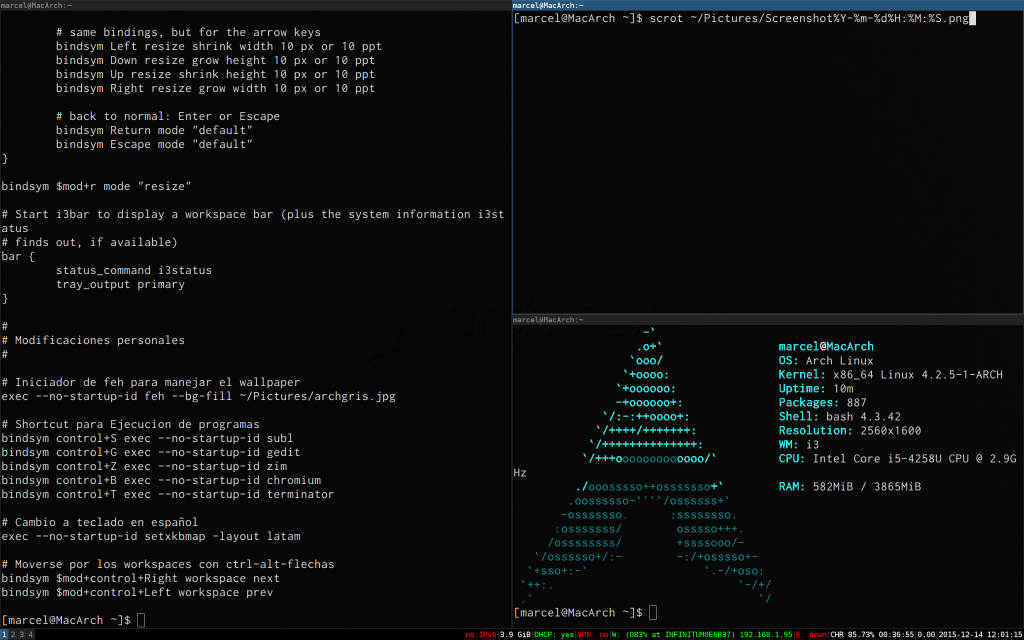
\includegraphics[width=1.15\textwidth]{./graphics/i3-desktop}}
\end{frame}

\begin{frame}{Why \ithree?}
    \ithree is awesome because:
    \begin{itemize}
        \item Vim bindings
        \item workspaces are first-class citizens
        \item opening terminal emulators is optimized
        \item highly customizable
    \end{itemize}
\end{frame}

\begin{frame}{Using \ithree}
    \begin{itemize}
        \item \texttt{Mod + Enter}: Open a terminal
        \item \texttt{Ctrl + D}: Open dmenu, a program launcher
        \item \texttt{Mod + \#}: move to workspace \texttt{\#} (\texttt{\#} $\in
            {0,\dots,9}$)
        \item \texttt{Mod + Shift + \#}: move current window to workspace
            \texttt{\#}
        \item \texttt{Mod + H/J/K/L}: make active window the one to the
            left/below/above/right, just like Vim.\footnote[frame]{I think by
            default it is actually shifted one to the right but that's fixable}
            You can also use the arrow keys.
        \item \texttt{Mod + Shift + H/J/K/L}: move window left/below/above/right
        \item \texttt{Mod + E}: activate split mode (default)
        \item \texttt{Mod + W}: activate tabbed mode
        \item \texttt{Mod + S}: activate stacked mode
        \item \texttt{Mod + Shift + Space}: float the current window
    \end{itemize}
    \hspace{1em}
\end{frame}

\begin{frame}[standout]
    \Huge
    Quick Live Demo
\end{frame}

\begin{frame}{Customizing \ithree}
    You can customize \ithree editing \texttt{.config/i3/config}.
    \begin{itemize}
        \item Desktop Background: \texttt{exec\_always feh --bg-fill <file>}
        \item Fonts: modify \texttt{font pango:<font>}
        \item Mod Key: \texttt{set \$mod Mod\#} (be careful or you could set it
            to the wrong key)
        \item Workspace Icons: \texttt{set \$workspace1 "1: \&\#xf269;"} results
            in a "1: \faFirefox"
    \end{itemize}

    You can customize the \texttt{i3status} bar by editing the
    \texttt{.config/i3status/config}.
\end{frame}

\begin{frame}{Installing \ithree}
    \begin{itemize}
        \item Arch: \texttt{pacman -S i3-wm i3status i3lock} (\texttt{i3lock} is
            optional)
        \item Ubuntu: \texttt{apt install i3}
        \item Gentoo: good luck
        \item Windows or macOS/OS X: install Linux
    \end{itemize}

    Then add \texttt{exec i3} to your \texttt{\textapprox/.xinitrc}.
\end{frame}

\begin{frame}{Further Reading}
    \begin{itemize}
        \item My configurations: \url{http://www.the-evans.family/sumner/.config/}
        \item The great \ithree docs: \url{https://i3wm.org/}
        \item You can also check out $\text{\texttt{i3-gaps}}^{\text{AUR}}$
    \end{itemize}
\end{frame}

\begin{frame}[standout]
    \Huge
    Questions?
\end{frame}

\end{document}
